% Chapter 2

\chapter{项目需求分析} % Main chapter title

\label{Chapter2} 
\section{用户背景介绍}
智慧足迹数据科技有限公司是中国联通集团控股,由中国联通和西班牙电信合资成立的专业大数据公司,依托中国联通卓越的数据能力、全球最强大的手机信令处理平台Smart Steps等产品技术和丰富的市场经验,提供位置信息洞察及相关大数据业务。\\
\indent 公司坚持对接国家战略,践行社会责任,落实集团关于大数据布局的战略思想,以“开垦、开放、开源”为发展战略,树立了“简单,成事”的企业文化,广泛集聚百度、高德、微软、Oracle、Teradata、HP、IBM、科研院所等国内外一流人才,打造了一支激情创业、价值导向、高效运营的大数据精英团队。\\
\indent Smart Steps是全球领先的位置大数据技术,利用匿名、聚合、外推的网络数据,经过高度自动化和深度降噪处理,将运营商数据加工成反映用户空间行为的时空标签,快速高效提供高价值的“线下位置+线上行为”的数据洞察服务。\\
\indent 公司通过“T”型产品战略赋能产业生态,横向开放合作,结合外部智脑综合利用数据,实现数据增值;纵向垂直应用,为行业客户提供全方位服务。公司以中国联通4亿+用户数据为基础,整合运营商、互联网、政府及商业等数据,采用AI化、标签化、模型化数据处理技术,自主研发10大产品平台,包含数据产品(统计数据集、统计数据API、能力开放DaaS平台、Data lab)、行业垂直产品(数据报告、实时热力及产业经济平台、数据可视化平台、极目洞察选址SaaS平台、金融风控平台、数字营销平台)等。\\
\indent 智慧足迹公司业务主要涵盖两个方面,分为产品平台和行业方案,这两者呈现相辅相成的关系,基于强大的信令数据资源和数据处理能力构建多元化的大数据平台,为不同需求的客户根据其不同的需求从不同的角度分析数据得出个性化的分析结果,从而得到不同行业解决方案。\\
\indent 数据平台分为数据智能平台,数据洞察平台,能力开放平台,数据引擎平台。其中数据智能平台中的统计数据集是基于联通用户的行为轨迹以及属性标签,通过SS平台的脱敏加工后,结合客户需求,实现不同时空、用户属性视角下的数据统计。产品以Excel或者CSV表格的形式对外提供(可选制图与报告配套销售),内容为统计数据集,客户可基于数据结果直接进行问题的研究以及分析决策。产品的主要功能是职住娱的分布、通勤和游憩、全目的的出行、人口动态变化、跨省跨域迁徙等。统计数据API将城市以250M边长的网格均匀覆盖,以接口调用形式访问,提供每一网格(或区域)各维度的人群特征属性,为进一步开展商业洞察、选址分析、指数评估、潜客挖掘提供数据依据。产品功能主要有基础人流数据、人群画像数据、人群流动数据、人群社会属性数据等。\\
\indent 极目洞察选址SaaS平台归属于数据洞察平台,通过简洁友好的交互界面,帮助客户快速监测定点区域周边客群资源,包括:客群规模、驻留特征、客群结构、消费能力、手机终端品牌、互联网偏好特征等;并基于行业模型为增量布点选址提供大数据决策支持。主要功能有,批量点洞察,自定义区域洞察,特定客群分布,自动推荐点位,定位评估等。实时热力及产业经济平台基于手机信令的实时热力产品是通过对手机信令进行实时处理和计算、分析,得出指定区域的实时人口特征,包括区域人口热力分布、人口数量、人口结构、人口来源、人口画像、人口迁徙、职住等信息。提供的产品形态包括:API数据接口或web页面。可为政府人口统计、应急监控及实时客流分析提供有价值的决策依据。主要功能有区域人口统计,人口流动统计,人口实时热力,区域人口结构,区域人口画像,人口职住分析等。数字营销平台依托中国联通的海量数据以及位置标签能力,在确保数据隐私安全的前提下,通过大数据的深入挖掘和分析为各行业客户优化投放策略和渠道,提供精准的营销触达手段。主要功能有标签定制,标签筛选,内容定制,营销策略定制,渠道灵活选择,营销监控,盘点及评估。金融风控平台在充分保障用户隐私安全的前提下,金融风控平台利用联通数据资源优势和领先的数据建模能力,提供反欺诈、信息核验和风险评估服务。帮助合作伙伴解决事前预防、事中防控、事后失联客户复联等业务流程相关的风险控制问题,达到降低业务风险,避免损失的效果。产品功能包括,职住验证,实时位置比对等。\\
\indent 数据能力开放DaaS平台,基于海量的联通多维数据,采用Hadoop大数据生态体系搭建集群,支持Spark、Hive等多种大数据挖掘及建模技术的应用。为客户提供基于位置的洞察、选址、营销等数据分析服务。平台用户可以通过接口的形式,运行各类定制化数据模型,安全合规的获取维度丰富的统计数据集结果,以满足行业应用的需求。产品功能主要有,区域洞察,客群发现,自主建模,主要可用于商业地产洞察,零售店选址,户外媒体点位洞察等。大数据可视化平台是公司自主研发的大数据产品,采集中国联通全国用户的手机信令数据和CRM系统属性数据,通过数据清洗、加工、处理和挖掘,运用领先的可视化技术,直观呈现海量数据隐含的巨大价值,提供人口监测与疏解、交通规划、公共安全、市场洞察等多样化决策支持。主要功能有人口分布,出行分析,跨域迁徙路线,区域人口洞察,选址分析,人流预警,可用于城市规划+智慧城市,职住分布+OD分析。\\
\indent 此外在数据引擎平台,还提供位置标签,即经SmartSteps信令处理平台加工,表达用户特征并满足客户需求的的集合数据。 AI业务模型:基于多源数据,利用机器学习等大数据技术和算法,构建行业场景应用模型。以及AI业务模型,基于多源数据,利用机器学习等大数据技术和算法,构建行业场景应用模型。\\
\indent 行业方案主要提供一下四个方面的服务,城市规划,政府治理,商企洞察,金融风控。城市规划设计人口分布分析,城市出行分析,城市间跨域迁徙分析,城市产业经济分析等。公司目前已经有两项成功案例,武汉市城市规划居民职住分析项目,协助武汉市政府全面了解武汉居民职住平衡比,评估各个区域发展规划是否合理。目前的初步识别结果为武汉市居住人口为1061万人,工作人口542万人,总体职住比为0.51。就各区的职住比而言,江汉区的职住比最高,武昌区,、青山区、东西湖和蔡甸区次之。金融街地区人口特征分析,协助金融街道办事处准确掌握在金融街居住的人在哪儿工作,以及工作的人在哪儿居住,为街区的合理规划提供依据。从工作人数的日变化来看,金融街地区人员集中在工作日期间,周末人员数量仅为工作日的26\%。金融街地区的就业者中,居住地在周边街道的居多,也有在房山、回龙观等地的。金融街地区的居住者中,在周边就业的居多。\\
\indent 由于随着国家经济快速发展城镇化率持续上升,除去“京津冀”“长三家”“珠三角”三大经济城市圈之外致力打造10大国家中心城市都市圈。并且,国家对高铁线路的加大投资使得人们在城市之间的流动更加边界,极大的促进升级、区域级包括经济、旅游、探亲等人口之间往来联系强度。引发了我国城市的居住与就业空间格局发生了深刻演变,城市规模明显扩大、城市用地日趋紧张,交通拥堵日益严重。作为城市居民生活与生产的两大载体,“居住”与“就业”是城市空间结构中的两个核心内生变量,它们彼此依存、互相影响,两者是否均衡发展是影响城市居民生活幸福指数的关键指标,制约城市可持续发展的重要因素。城市工作人口、流动人口、居住人口的等不同类型的居民对政府各个单位的诉求千差万别。社会治理面临巨大挑战,政府传统服务方式已经难以满足。因此,采用大数据技术对海量数据快速收集与挖掘为社会治理、推动就业与居住均衡发展把握城市发展规划,促进居住空间与产业空间拓展的联动与共赢显得非常必要。可以协助解决诸如人口规模分析,人口结构分析,人口实时监测,人口专题分析,城市交通干线流量分析,城际交通路网通行效率评估,城市交通运营与分析,游客洞察,游客营销等。典型案例有北京市统计局人口统计项目,北京市委十一届七次全会通过了《关于贯彻落实《京津冀协同发展规划纲要》的意见》,明确了人口发展目标和加强人口调控的具体要求,疏解非首都功能,加强人口数据的动态监测。《京津冀协同发展规划纲要》中明确了北京2300万的人口控制目标,是为人口调控的红线不能突破。因此,如何有效调控人口规模,精确掌握人口流向,及时预警特殊区域人口聚集建立北京市人口动态监测平台成为人口统计工作的重点。基于北京联通手机用户信令数据分析的人口动态监测平台可以实时统计北京市辖区人口热力分布,也可出具日度、周度、月度、季度、年度等不同时间周期的人口统计报告。为北京市政府的人口统计、调控、监控提供有效数据支持。提升区域人口管理及监测的工作效率,合理制定政府疏解政策。商企洞察包含区域客群洞察,商业选址评估,户外媒体分析与监测等方面。成功案例有,某知名地产研究机构城市人群洞察研究,通过精准的大数据分析,对城市区域进行量化分析,形成新店建设建议;并可对已建商铺(营业厅、连锁店)进行量化评估,找出分值高和分值低的商铺。某知名连锁超市企业全国门店选址服务,为某知名连锁超市企业提供新建门店的洞察选址服务,通过便捷交互、清晰展现的可视化SaaS服务,基于联通用户属性数据及线下行为数据,快速识别目标客群城市内线下聚集区域,并进而通过区域客群洞察对比找出最适合建店的区域,实现“量化”选址,大幅提升了超市选址的效率与准确性,并节约了大量的人力成本和时间成本。某大数据广告服务商30个城市数万个户外媒体点位监测,为某新兴O2O传播整合营销公司,长期提供30个城市(包括北上广深、14个省会城市、12个大型城市)的万余指定线下媒体资源点位辐射区域的连续、准确的客群洞察监测服务,有效地解决了户外媒体点位价值评估与潜客定位的难题。同时,基于目标人群特征筛选,输出特定群体在指定城市的分布,帮助该企业为广告主提供有针对性的O2O落地营销方案。金融风控服务是全面整合多维、合规和完整的多家运营商大数据,为金融机构提供客户信息验证、号码风险评估、号码消费情况、手机终端型号查询和信用分等运营商风控数据服务。结合智慧足迹的精准位置定位、完整轨迹画像和长期洞察,为客户提供实时位置差,历史位置比对、职住验真等运营商位置服务。成功案例有银行及其他金融机构风控服务,银行客户通过采购运营商数据,实现银行各业务部门信贷审批的欺诈风险、信用风险管控。为银行提供三要素验证、二要素验证、在网时长、号码归属地、手机状态等信控数据接口,帮助银行验证客户风险。并对接月消费档次、是否历史欠费、终端机型、实时位置查询、历史位置验证等,为银行提供了全面丰富的运营商维度的征信风控数据验证服务。某大型互联网金融公司,为某top互联网金融公司提供三要素验证、二次卡验证、手机号状态、在网时长、话费评分、话务量评分、流量评分等征信接口服务;并基于联通能力开放平台,对话单及位置数据进行挖掘,进一步提供用户风险属性特征服务;服务于包括消费金融、钱包支付、互联网证券、互联网银行、互联网保险等业务的多个板块。某银行精准营销项目,某银行在提供用户授权协议的条件下,提供身份核实、黑名单用户查询、实时位置查询、最后一次活跃用户查询等数据服务。使得银行快速筛选定位目标用户群,并通过联通公司的多渠道方式进行用户直达,快速实现获客。
\section{用户需求分析}
人口规模和分布一直是城市规划、 城市管理领域关注的核心问题,尤其是在我国城镇化进入下半场, 人才争夺日益激烈的今天。传统的预测模型多是对于规模的预测,而对人口的时空分布关注较少,总
量预测固然意义很大,但空间分布的重要性也不容小觑。 本项目拟利用智慧足迹公司掌握的某区域近1年的手机信令数据,并结合外部网络公开数据,
在标定不同时段人口分布的基础上,构建合适的模型,实现对周、 小时等
空间粒度,乡镇、 网格等时间粒度的人口分布预测,并评估其可靠性,以
期为城市的监测、 预警等精细化管理,以供参考。\\
\indent 总结而言,就是通过历史的人口时空分布数据,来预测未来的人口时空分布。具体说的话,通过北京六环以内,1km网格尺度的分天分小时人口分布数据(历史数据的时间跨度可以拉长到3个月)预测未来一周 相应网格下每天每小时的人口分布。
\section{市场前景分析}
\subsection{信令数据分析相关案例和技术应用场景}
\subsubsection*{手机信令数据的分析价值}
作为城市活动的参与主体,了解人口活动的分布和规律通常是一个城市所有问题的基础。越来越多的城市管理者和规划师已经意识到人作为重要主体在城市中的重要性。而在城市规划中,“人”的监测难度较大,通过传统人口调查的静态获取数据方式很难得到及时的信息。故而,可以提供用户空间位置的手机信令信息让人口移动的实时检测和分析成为可能。
\subsubsection*{手机信令数据商业化的应用场景}
\begin{itemize}
	\item 国外数据使用案例:\\
	美国电信运营商Verizon成立了精准营销部门Precision Marketing Division。该部门提供精准营销洞察(Precision Market Insights),提供商业数据分析服务。如在美国,棒球和篮球比赛是商家最为看中的营销场合,此前在超级碗和NBA的比赛中,Verizon针对观众的来源地进行了精确数据分析,球队得以了解观众对赞助商的喜好等;美国电信运营商Sprint则利用大数据为行业客户提供消费者和市场洞察,包括人口特征、行为特征以及季节性分析等方面。
	\item 国内数据使用案例 \\
	深入了解具有特定偏好的人群的时空分布特征,找到满足目标客群触达(条件)的户外媒体点位。按照智慧足迹标签分类体系(用户自然属性、时空属性、互联网偏好属性等),筛选用户群体,发现目标客群的常驻地(居住、工作等)分布。
\end{itemize}
\subsubsection*{基于大数据的监测和决策支撑服务}
\begin{itemize}
	\item  国外数据使用案例:客流和选址\\
	西班牙电信于2012年10月成立了动态洞察部门DynamicInsights开展大数据业务,为客户提供数据分析打包服务。该部门与市场研究机构GFK进行合作,在英国、巴西推出了首款产品名为智慧足迹(Smart Steps)。智慧足迹基于完全匿名和聚合的移动网络数据,帮助零售商分析顾客来源和各商铺、展位的人流情况以及消费者特征和消费能力,并将洞察结果面向政企客户提供客流分析和零售店选址服务。
	\item 国内数据使用案例:基于大数据的北京城市副中心典型问题研究\\
	项目紧扣北京城市副中心规划、建设和管理的目标与现实问题,旨在采用手机信令、企业、POI、公交一卡通等多源大数据,建立针对北京城市副中心建设发展过程典型问题的指标体系,并从产业、人、交通、房屋和设施五个方向进行归纳、评估、分析,把握问题演变特征、挖掘认识发展规律,为北京城市副中心建设发展提供决策参考。
\end{itemize}
\subsection{智慧足迹和竞争对手分析}
\subsubsection*{智慧足迹历史和发展}
中国联通智慧足迹座位中国位置大数据应用的第一服务商,是中国联通集团控股,由中国联通和西班牙电信合资成立的专业大数据公司,依托中国联通卓越的数据能力、全球最强大的手机信令处理平台Smart Steps等产品技术和丰富的市场经验,提供位置信息洞察及相关大数据业务。智慧足迹在
公司通过“T”型产品战略赋能产业生态,横向开放合作,结合外部智脑综合利用数据,实现数据增值;纵向垂直应用,为行业客户提供全方位服务。城市规划、商企洞察选址、金融位置应用垂直领域取得了领先地位。支撑国家七大部委及重点省市政府,提供200多个城市规划统计数据集服务,市场占有率80\%,成为信令位置数据应用第一服务商。
\subsubsection*{智慧足迹相关竞争对手及对手}
见表格\ref{table:1}
\begin{table}
\centering
\caption{智慧足迹相关竞争对手及对手}
\label{table:1}
\begin{tabular}{p{0.2\columnwidth}|p{0.2\columnwidth}|p{0.2\columnwidth}|p{0.2\columnwidth}}
\hline
\hline
联通智慧足迹 & 上海数慧 & 清华同衡 & 晶众股份\\
\hline
位置大数据应用提供商&大数据在城市规划应用服务商&传统和创新并进的规划设计院&大数据交通应用服务商\\
\hline
\hline
\end{tabular}
\end{table}
\section{数据预处理和分析}
\subsection{数据清洗}
\subsubsection*{确定基站编号与地理位置间的关系}
之所以我们需要得到基站与网格分布的对应关系,是因为每个网格的人口数据不仅是时序的,还与空间分布有关。例如某网格人数的增加与周围网格人数减少相关。前期的数据预处理得到网格分布可能为后续预测提供方便。\\
\indent 原始的基站编号为 wkt 坐标,通过分析原始数据发现基站的编号不是从零开始连续的,说你有一些位置(山地、河流)等没有人流量的数据;而原始的数据只给出了基站编号对应的 wkt 坐标数据,需要处理得到基站编号基站位置分布的关系,如图\ref{fig:2.1}所示。
\begin{figure}[ht]
\centering
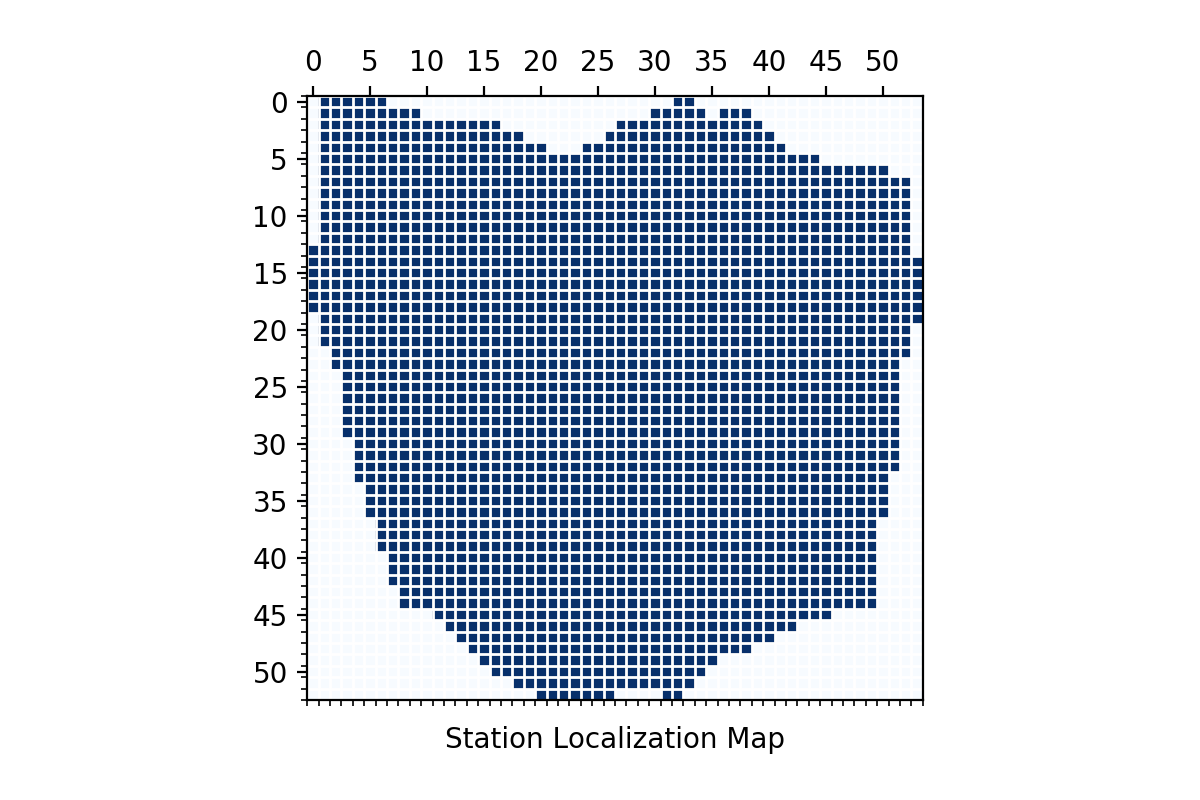
\includegraphics[width=\textwidth]{station_location.png}
\caption{基站位置分布图}
\label{fig:2.1}
\end{figure}
图中显示,基站所覆盖区域被基站划分为54行53列的网格,对应2862个基站,且基站编号从网格左上角开始从左到右从上到下依次加一。图中红色网格代表提供人口流动数据的基站,蓝色网格则是无人区域。\\
\indent 基于此处理基站与网格分布关系,得到三个表格待后续分析使用:
\begin{itemize}
	\item基站编号---网格行列转换表
	\item 网格---基站编号转换表
	\item 无人区基站编号表
\end{itemize}
\subsubsection*{数据结构化、添补数据缺失}
数据范围是2017年9到11月人口流动数据。每天分24小时记录数据,每一行给出某天第几个小时第几号网格的,驻留人数、出发及到达人数。
为了便于后续数据处理,将数据形式进行处理。以驻留人数为例,每行表示某天某小时的所有基站数据,共2862列。无人区补零。
还有很少数的基站在一些时间点有数据缺失的情况,用该时刻前或后一时刻的数据填补。
\subsection{预处理和分析}
\subsubsection*{人流变化的短周期性}
观察以(15,30)为中心25个网格的一周内人口数量变化(见图\ref{fig:2.2}):
\begin{figure}[ht]
\centering
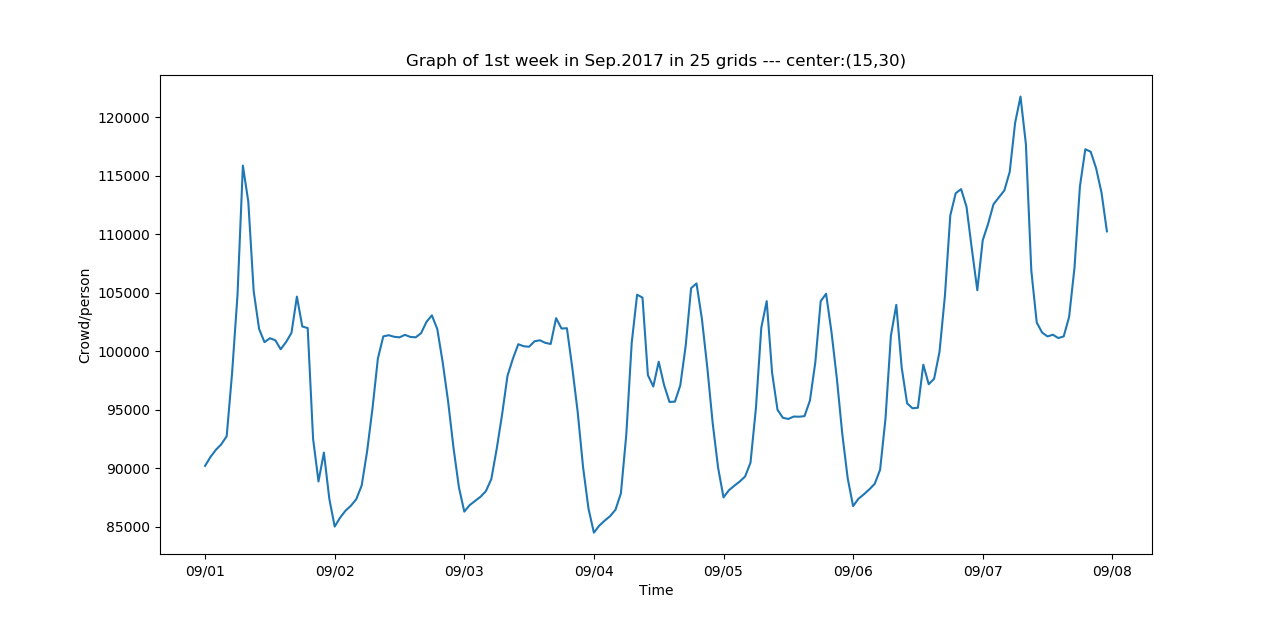
\includegraphics[width=0.8\textwidth]{month9_week1_25grids.png}
\caption{25个网格内人流一周内变化}
\label{fig:2.2}
\end{figure}
之所以取25个网格观察,是希望弱化网格间人口流量的影响,主要观察时序变化规律。
\indent 可以发现:
\begin{enumerate}
	\item 每天的人口驻留数量有明显的周期性变化。凌晨左右的人口数量最低。
	\item 已知09/02和09/03是周末,发现周末的人口数据与周中人口数据有所不同。
\end{enumerate}
\subsubsection*{人流变化的长周期性}
观察以(15,30)为中心25个网格的三周内人口数量变化,图(\ref{fig:2.3})中红线代表每周周六,可以看到人口数量在各周间也有所波动。
\begin{figure}[ht]
\centering
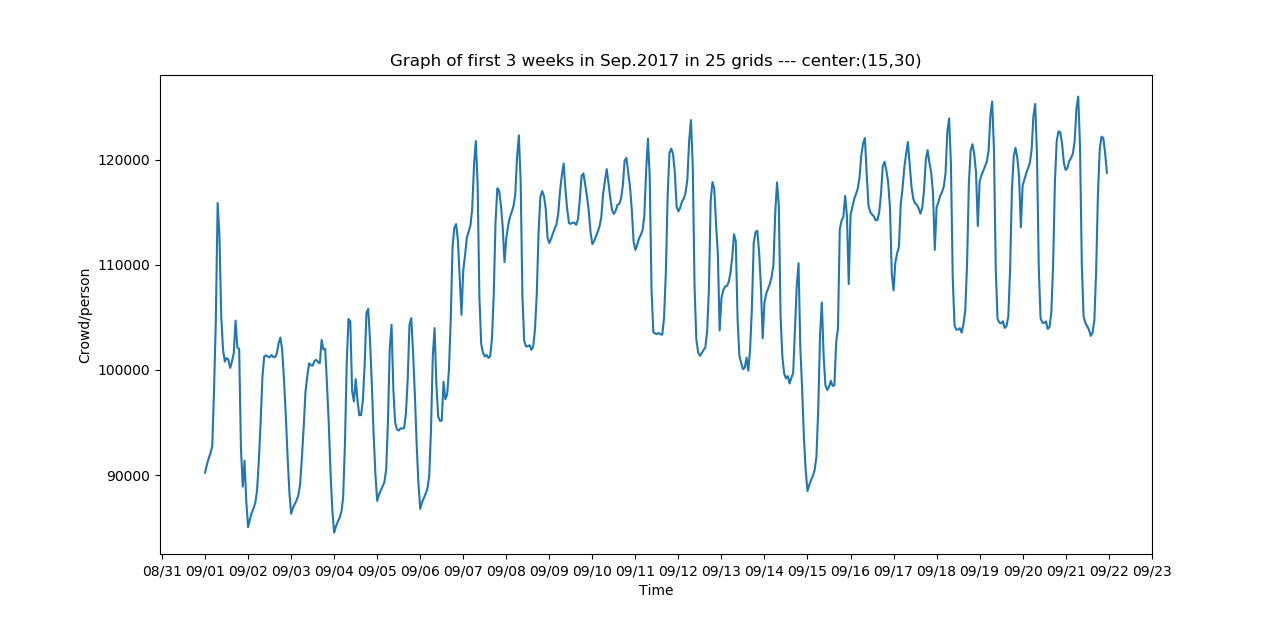
\includegraphics[width=0.8\textwidth]{month9_week3_25grids.png}
\caption{25个网格内人流三周内变化}
\label{fig:2.3}
\end{figure}
\subsubsection*{相邻地域的关联性}
以(15,30)(15,31)两个网格一天的人口流动为例,可以观测网格位置关联的地域的人流相关性。
\begin{figure}[ht]
\centering
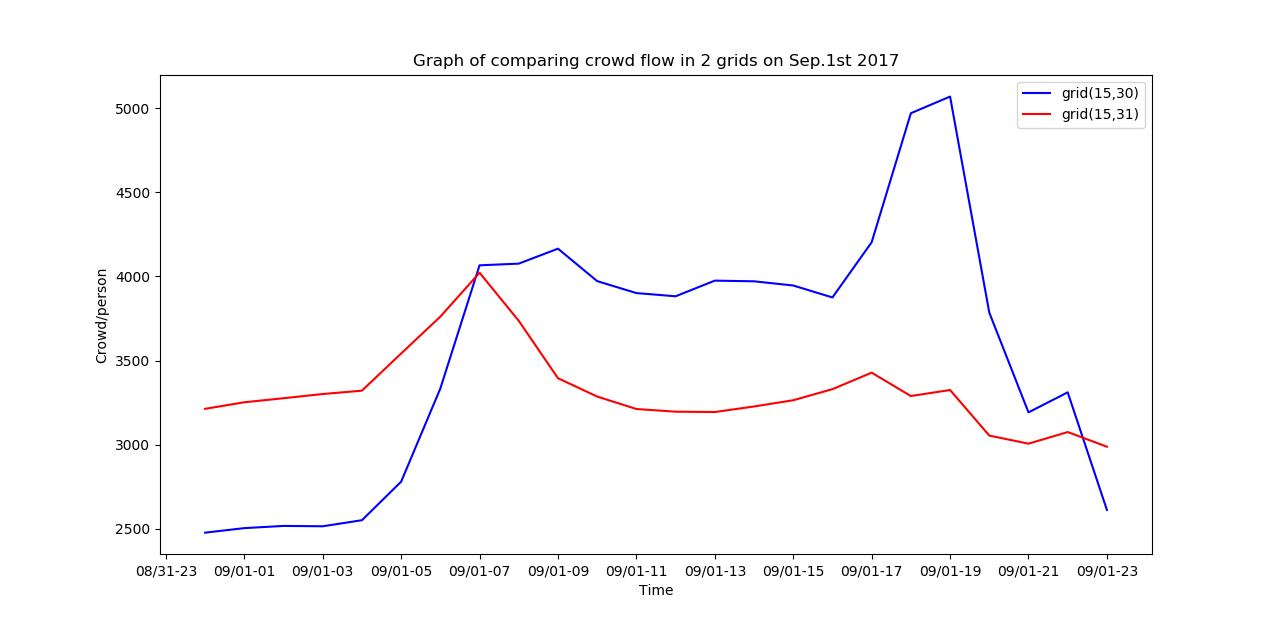
\includegraphics[width=0.8\textwidth]{compare.png}
\caption{两个相邻网格一天的人口流动}
\label{fig:2.4}
\end{figure}
\indent 从图(\ref{fig:2.4})中,
观察绿色框,可以发现一个网格人口增多另一个网格人口减少,其原因可能与人们在这两地移动相关,这在一定程度上体现网格位置对人口流动的影响。
\section{技术方案选择}
\subsection{可选技术方案}
\subsubsection*{ARIMA时序数据预测方法}
对于非平稳的时序序列,常常可以采用差分自回归移动平均模型(Autoregressive–moving-average model,ARIMA)进行分析\cite{whittle1966prediction,Hannan1970Multiple}。
在ARIMA(p,d,q)模型中,p 代表自回归阶数,d 代表差分次数, q 代表移动平均阶数,这一模型的建立需要解决以下三个问题:
\begin{enumerate}
	\item 利用差分将非平稳序列转化为平稳序列
	\item 通过模式识别确定模型属于AR、MA、ARMA中的哪一种
	\item 通过模式识别确定模型属于AR、MA、ARMA中的哪一种
\end{enumerate}
\indent 基于此,一种简单的预测方式可以对每个网格的时序序列进行建模求解,得到初步的预测情况。但是,网格的数量有两千两百多个,求解的计算量是较大的。同时,这样一来便没有考虑网格的位置分布关系对人口流动的影响。\\
\indent 基于这一模型的特点,比较适用于对于一些感兴趣的网络进行初步近似求解。
\subsubsection*{Res-CNN方法}
有文献\cite{Zhang2016Deep}指出,对于试图预测的某一时刻人口数量,在时序上,受到3个部分的影响:
\begin{itemize}
	\item $X_c$邻近时刻(例如之前的几个小时)
	\item $X_p$周期(例如昨天、前天的同一时刻)
	\item $X_q$趋势(例如上周、上上周等的同一时刻)
\end{itemize}
所以可以利用相同的网络结构来处理以上三部分信息。
\indent 另外,由于卷积层CNN通过卷积核的扫描融入了网格分布的位置信息,多个卷积层的叠加又可以使特征层次有小到大,所以文章先利用CNN对信息进行处理。
为了改善卷积层过深梯度消失的问题,在卷积层后加入了残差网络Res\ref{fig:2.5},从而构成了时序部分的网络结构。
\begin{figure}[ht]
\centering
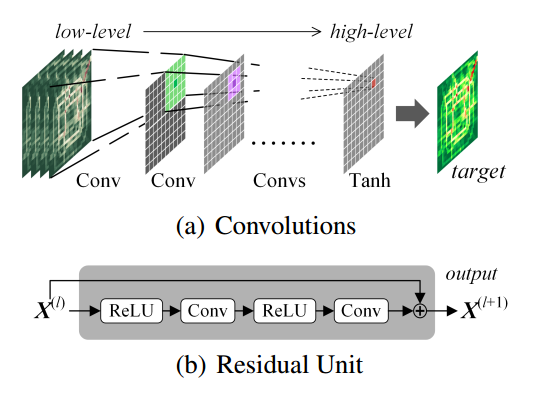
\includegraphics[width=0.8\textwidth]{Residual.png}
\caption{卷积层和残差单元}
\label{fig:2.5}
\end{figure}
最后,三个相同结构网络得到的数据,通过与参数矩阵相乘再相加的方式进行融合与维度的统一。同时训练得到了矩阵中的参数。
\\
\indent 另外,还可以考虑外部因素$E_t$(如天气等)对于人口流动的影响,其最终的网络结构如图(\ref{fig:2.6})所示。
\begin{figure}[ht]
\centering
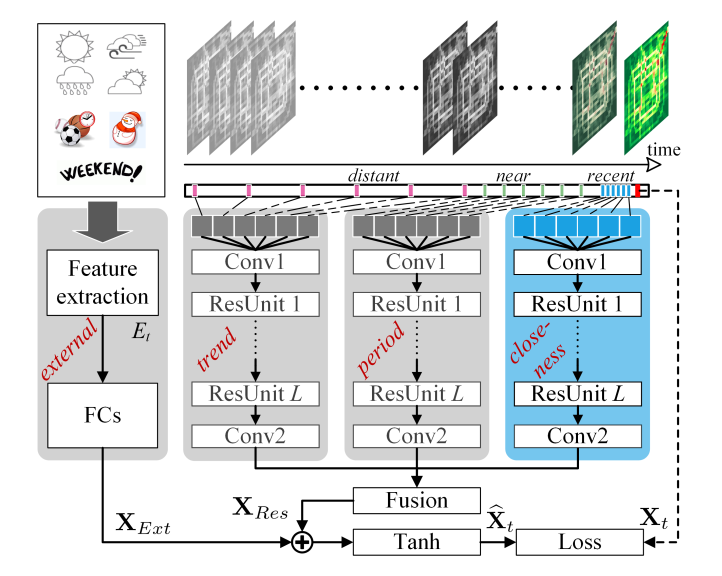
\includegraphics[width=0.8\textwidth]{net.png}
\caption{网络结构}
\label{fig:2.6}
\end{figure}
其中左侧是处理外部因素的,右侧是3个相似的卷积残差网络用来处理时序数据。将$E_t$转变成对应的特征向量,在其后连接两个全连接层FC。第一个全连接层可以看作对特征的提取,第二层则是为了获得与时序数据处理结果有相同维度。两部分最后的融合方式直接相加,并通过双曲正切函数控制在(-1,1)之间。网络的损失函数为预测与实际值误差的平方:
\begin{equation}
Loss = \Arrowvert y_t - \hat{y_t} \Arrowvert^2
\end{equation}
